Известный психолог педагог Бенжамин Блум в работе \сite{bloom1984} изучает проблемы массового образования.
Согласно его исследованию индивидуальное образование позволяют получать 
результаты в пределах до двух сигмах лучше общего образования. Для разрешения проблемы
предлагаются методы, основанные на нейропсихологии


\textit{Определение} Индивидуальная образовательная
траектория 

Отличается от персонализированного обучения, в котором траекторию своего обучения определяет сам учащийся, тем, 

что в этом случае в формировании образовательной траектории участвуют педагоги.






\textit{Определение} \textbf{Дидактический подход} ориентирован на . 
 
Акцент при обучении ставиться на контроле за успеваемостью учащихся, 
регулярно проводятся контрольные занятия, представляющие количественную оценку знаний и навыков.
Курсы как правило сопровождаются подготовленной средой: учебником, рабочей тетрадью и лабораторной установкой.

Особенность обучения заключается в прямом участии учителя в работе.

Минусами такого подхода служит необъективность отбора материала,
отсутствие возможности учащегося повлиять на материал обучения, 
потребность в значительной подготовке преподавателя к занятию и ежегодной закупки расходных методических материалов.

Противопоставленным дидактическому методу обучения является проблемно-ориентированный подход.
в отличие от дидактического подхода, который акцентирует внимание на передаче знаний от учителя к ученику,
эмпирический подход ставит в центр обучения активное участие ученика в исследовании
и поиске знаний через решение проблем и практическую деятельность.
Этот подход поддерживает самостоятельное мышление, исследовательские навыки и обучение через самостоятельное осмысление опыта.
Ученики, таким образом, сталкиваются с реальными проблемами или задачами, 
ищут способы их решения, экспериментируют и совместно с учителем извлекают уроки из этого опыта.
Эмпирический подход часто ассоциируется с \textit{активными методами обучения}, описанными в работах Кругликова \cite{кругликов2006деловые}

\begin{itemize}
    \item Решение казусов
    \item Исследовательские проекты
    \item Командная работа
\end{itemize}

\textit{Определение} Практико-ориентированный подход подразумевает приобретение знаний
 с помощью выполнения задач, приближенных.

Такое обучение основано на принципе активного участия, где ученики самостоятельно формулируют и анализируют проблемы, 
 разрабатывают стратегии исследования и находят решения. 
 Учитель выступает скорее в роли наставника, который поддерживает 
 и направляет учащихся в процессе решения проблемы, обеспечивает необходимую информацию и
 стимулирует критическое мышление и самостоятельность.


\begin{figure}[h]
    \centering
    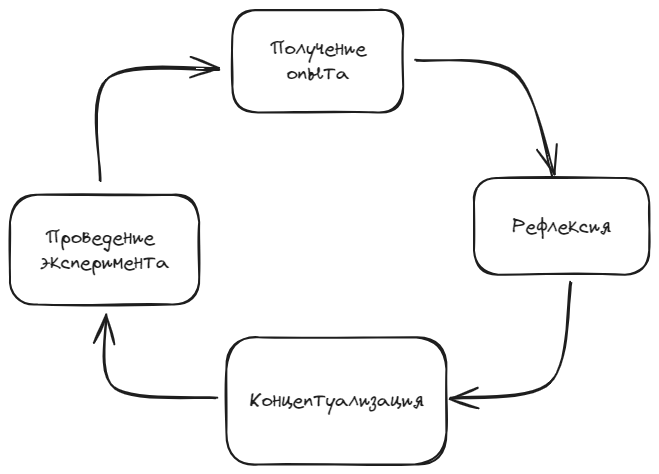
\includegraphics[width=0.5\textwidth]{assets/pedagogic/colb.excalidraw.png}
    \caption{Цикл Колба}
    \label{colb}
\end{figure}

Одной из известных моделей является цикл Колба \cite{kolb2014experiential}



Организация исследовательских проектов предполагает создание структурированной и поддерживающей среды, в которой учащиеся могут самостоятельно исследовать определенную тему или проблему. В ходе организации таких проектов важно определить ясные цели и задачи исследования, а также обеспечить доступ к необходимым ресурсам и информации. Учитывается также выбор соответствующих методов исследования и инструментов для сбора и анализа данных. Кроме того, организация исследовательских проектов включает в себя установление сроков и этапов работы, распределение обязанностей между участниками команды и создание механизмов обратной связи и поддержки. Это позволяет учащимся эффективно планировать и осуществлять свои исследовательские усилия, развивать навыки самоорганизации, анализа и критического мышления, а также получать удовлетворение от процесса открытия новых знаний и исследовательской деятельности.

Оценка исследовательского проекта требует объективности и учета нескольких ключевых аспектов. Один из подходов - это использование критериев оценки, которые определяются заранее и включают различные аспекты проекта, такие как оригинальность идеи, методология исследования, анализ данных, качество презентации и выводов. Каждый критерий может быть оценен на числовой шкале, что позволяет сделать оценку более объективной.

В рамках конкурса исследовательских проектов могут быть применены различные техники для оценки работ участников. Одна из таких техник - это использование экспертных жюри, состоящих из опытных специалистов в соответствующей области, которые могут оценить проекты с точки зрения их научной значимости, методологии и оригинальности идей. Другой метод - это организация публичных презентаций проектов, во время которых участники представляют свои исследования перед широкой аудиторией и получают обратную связь от зрителей и экспертов.

Также важно обеспечить прозрачность и справедливость процесса оценки, предоставив участникам обратную связь и объяснив критерии и принципы оценки заранее. Это поможет участникам лучше понять ожидания и требования к их проектам, а также повысит доверие к результатам конкурса.


Также существенно снижается скорость освоения материалов в следствие отсуствия
 структурированной обратной связи, явного примера для изучения и воспроизведения.

На практике подход к методическому курс состоит в совмещение дидактического и опытного подхода. 


Мерой успешности курса можно определить степень рефлексии учащихся на освоенный материал.

\textit{Определение}\textit{Рефлексия} в образовании играет значительную роль в 
стимулировании глубокого понимания и личностного развития учащихся. 
Этот процесс включает в себя осознанный анализ своего учебного опыта, 
рассмотрение своих мыслей, чувств и действий в контексте обучения.


\begin{figure}[h]
    \centering
    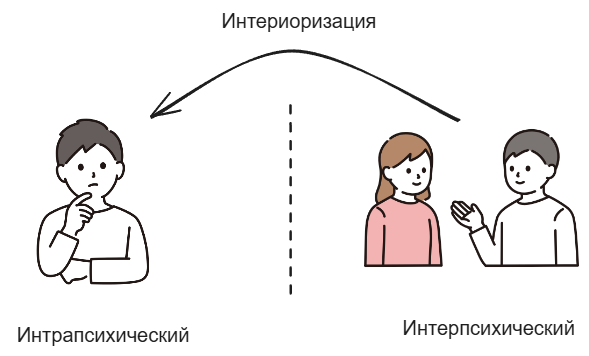
\includegraphics[width=0.5\textwidth]{assets/pedagogic/reflection.excalidraw.png}
    \caption{Рефлексия по Выготскому \cite{выготский2014мышление}}
    \label{reflection}
\end{figure}

Лев Выготский описывают рефлексию как результат интериоризации -
перехода внешней речи во внутренний способ мышления, когда ребёнок способен уже в уме планировать свою деятельность 

Рефлексия способствует развитию метакогнитивных навыков \begin{itemize}
    \item оценки своей деятельности и планирования
    \item осознания ценности знания и социума
    \item ведения высшей когнитивной деятельности по организации социальной деятельности
\end{itemize}
Таким навыки позволяют справляться с практическими заданиями, обучать и осваивать неизвестные областях знаний.

выявить собственные пробелы в знаниях и развить критическое мышление.


\textit{Определение} \textbf{Автодидактический} подход основан на самостоятельном обучении. 








